%!TEX root = W2b.beamer.tex

% Author: Sharon Nielsen
% University of Adelaide
%
%
%\documentclass{beamer}

\usetheme{Feather}
\setbeamercovered{transparent}

%\usecolortheme{orchid}
%\setbeamertemplate{background canvas}{\includegraphics	[width=\paperwidth]{code}}

\usepackage{hyperref}
\usepackage{multirow}
\usepackage{graphics}
\usepackage{epsfig}
\usepackage{verbatim}
\usepackage{fancyvrb}
\usepackage{shortvrb}
\usepackage{moreverb}
\usepackage[dvips]{rotating}
\usepackage{pifont}
\usepackage{tikz}
\usepackage{apacite}
\usepackage{booktabs}
\newcommand{\head}[1]{\textnormal{\textbf{#1}}}


\usepackage{setspace}
\usepackage{graphicx}
\usepackage{amsmath}
\usepackage{multicol}
\usepackage{wasysym}
\usepackage{colortbl}


\usepackage[light]{iwona}
\usepackage[T1]{fontenc}

\usepackage{listings}% http://ctan.org/pkg/listings
\lstset{
  basicstyle=\ttfamily,
  mathescape
}

\usefonttheme{professionalfonts}

\definecolor{mygrey}{gray}{0.7}


\title[W1 - Analysis]{W2 - Statistical Analysis of Agronomic Experiments}
\author{Sharon Nielsen, Bev Gogel}
\date{March 2018 \\ \vspace{0.2cm}\footnotesize  sharon.nielsen@adelaide.edu.au}




\begin{document}


%%%%%%%%%%%%%%%%%%%%%%%%%%%%%%%%%%%%%%%%%%%%%%%%%%%%%%%%%%%%%%%%%%%%%%%%%%%%%%%%%%%%%%%%%%%%%%%%%%%
% Slide
%%%%%%%%%%%%%%%%%%%%%%%%%%%%%%%%%%%%%%%%%%%%%%%%%%%%%%%%%%%%%%%%%%%%%%%%%%%%%%%%%%%%%%%%%%%%%%%%%%%
\begin{frame}[fragile]\frametitle{Exercise 5}
\begin{verbatim}
Response: EarInfect
          Df Sum Sq Mean Sq F value    Pr(>F)
row        4  83.62  20.906  3.4428   0.04287 *
col        4  24.77   6.193  1.0199   0.43576
Treatment  4 826.56 206.640 34.0302 1.842e-06 ***
Residuals 12  72.87   6.072

       EarInfect groups
Silk      48.118      a
Damage    43.518     ab
Stalk     38.952     bc
Seed      35.978     cd
Root      31.608      d
\end{verbatim}
\end{frame}

%%%%%%%%%%%%%%%%%%%%%%%%%%%%%%%%%%%%%%%%%%%%%%%%%%%%%%%%%%%%%%%%%%%%%%%%%%%%%%%%%%%%%%%%%%%%%%%%%%%
% Slide
%%%%%%%%%%%%%%%%%%%%%%%%%%%%%%%%%%%%%%%%%%%%%%%%%%%%%%%%%%%%%%%%%%%%%%%%%%%%%%%%%%%%%%%%%%%%%%%%%%%
\begin{frame}[fragile]\frametitle{Exercise 6}
\begin{verbatim}
Response: SugarYield
          Df  Sum Sq Mean Sq F value   Pr(>F)
row        3  11.778   3.926  1.0854 0.424093
col        3 101.145  33.715  9.3212 0.011231 *
Treatment  3 172.965  57.655 15.9398 0.002901 **
Residuals  6  21.702   3.617

    SugarYield groups
T0     24.3900      a
T12    21.4025     ab
T8     17.5100     bc
T4     16.0100      c
\end{verbatim}
\end{frame}


%%%%%%%%%%%%%%%%%%%%%%%%%%%%%%%%%%%%%%%%%%%%%%%%%%%%%%%%%%%%%%%%%%%%%%%%%%%%%%%%%%%%%%%%%%%%%%%%%%%
% Slide
%%%%%%%%%%%%%%%%%%%%%%%%%%%%%%%%%%%%%%%%%%%%%%%%%%%%%%%%%%%%%%%%%%%%%%%%%%%%%%%%%%%%%%%%%%%%%%%%%%%
\begin{frame}\frametitle{Linear Mixed Models}
The results from a linear model are reliant on the model assumptions being met and in all examples
investigated this was the case. In research there is data that do not meet these requirements, or
that are not complete, or arise from more complex experiments. These data can be analysed using Linear
Mixed Models (LMM) using much the same process as previously used. A LMM can be used instead of linear models, the
mathematics behind the model is quite different to a linear model but the results will be equivalent.
\end{frame}


%%%%%%%%%%%%%%%%%%%%%%%%%%%%%%%%%%%%%%%%%%%%%%%%%%%%%%%%%%%%%%%%%%%%%%%%%%%%%%%%%%%%%%%%%%%%%%%%%%%
% Slide
%%%%%%%%%%%%%%%%%%%%%%%%%%%%%%%%%%%%%%%%%%%%%%%%%%%%%%%%%%%%%%%%%%%%%%%%%%%%%%%%%%%%%%%%%%%%%%%%%%%
\begin{frame}\frametitle{Linear Mixed Models}
A LMM has combines two models into one, a \textbf{fixed model} and a \textbf{random model}.
The fixed is used to describe the explanatory structure of the experiment and the random is
used to describe the structural component of the experiment.

\vspace{0.5cm}

In the first part of this chapter some of the previous examples will be revisited and analysed using a LMM approach.
ASReml-R \cite{asremlr} is used as the tool to analyse the data using the function \texttt{asreml}.

\vspace{1cm}
\flushright

\includegraphics[height = 0.3cm]{yourturn}

\end{frame}


%%%%%%%%%%%%%%%%%%%%%%%%%%%%%%%%%%%%%%%%%%%%%%%%%%%%%%%%%%%%%%%%%%%%%%%%%%%%%%%%%%%%%%%%%%%%%%%%%%%
% Slide
%%%%%%%%%%%%%%%%%%%%%%%%%%%%%%%%%%%%%%%%%%%%%%%%%%%%%%%%%%%%%%%%%%%%%%%%%%%%%%%%%%%%%%%%%%%%%%%%%%%
\begin{frame}\frametitle{LMM - Example 3 revisited}
The linear mixed model that is fit can be symbolically written as:
\begin{eqnarray*}
	\texttt{Response variable}&:& \texttt{Yield} \\
	\texttt{Structural component}&:& \texttt{Block}\\
	\texttt{Explanatory component}&:& \texttt{Variety}\\
	\texttt{Residual}&:& \texttt{Assume independence}
\end{eqnarray*}

\vspace{1cm}
\centering
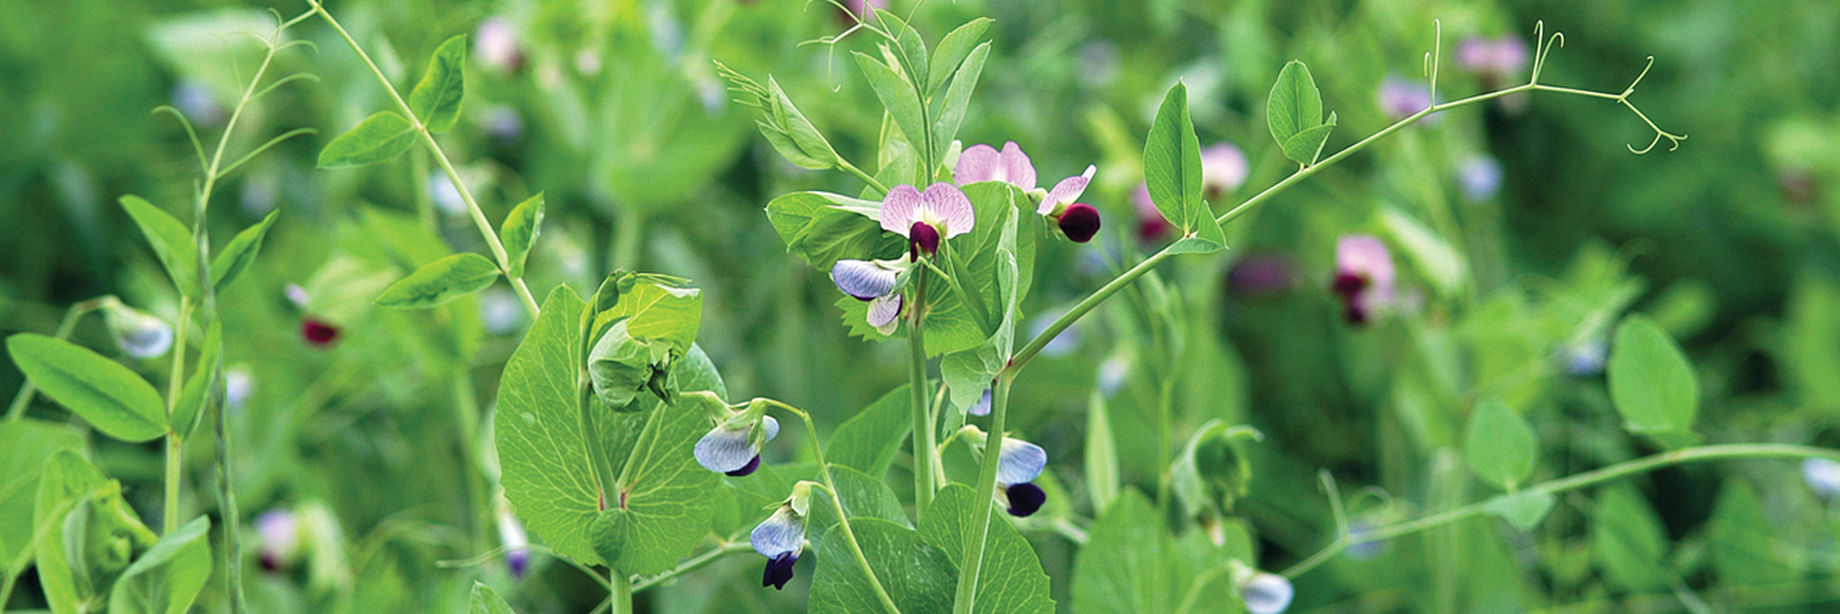
\includegraphics[width = 8cm]{fpeas}

\end{frame}


%%%%%%%%%%%%%%%%%%%%%%%%%%%%%%%%%%%%%%%%%%%%%%%%%%%%%%%%%%%%%%%%%%%%%%%%%%%%%%%%%%%%%%%%%%%%%%%%%%%
% Slide
%%%%%%%%%%%%%%%%%%%%%%%%%%%%%%%%%%%%%%%%%%%%%%%%%%%%%%%%%%%%%%%%%%%%%%%%%%%%%%%%%%%%%%%%%%%%%%%%%%%
\begin{frame}\frametitle{Likelihood-ratio test}
\begin{eqnarray*}
	H_0&:& \texttt{The reduced model is true or the dropped term is not significant} \\
	H_1&:& \texttt{The current model is true or the dropped term is significant}
\end{eqnarray*}


Here to test the null hypothesis that an arbitrary group of $k$ coefficients from the model is set equal to zero (e.g.
no relationship with the response), we need to fit two \textbf{nested} models, the:


\begin{enumerate}
\item \textbf{reduced model} which omits the $k$ predictors in question, and
\item \textbf{current model} which includes them.
\end{enumerate}
\end{frame}


%%%%%%%%%%%%%%%%%%%%%%%%%%%%%%%%%%%%%%%%%%%%%%%%%%%%%%%%%%%%%%%%%%%%%%%%%%%%%%%%%%%%%%%%%%%%%%%%%%%
% Slide
%%%%%%%%%%%%%%%%%%%%%%%%%%%%%%%%%%%%%%%%%%%%%%%%%%%%%%%%%%%%%%%%%%%%%%%%%%%%%%%%%%%%%%%%%%%%%%%%%%%
\begin{frame}\frametitle{Likelihood-ratio test}
The likelihood-ratio test is

\begin{eqnarray*}
\Delta = -2 \times logL \texttt{ from reduced model} - (-2 \times logL \texttt{ from current model})
\end{eqnarray*}


and the degrees of freedom is $k$ (the number of coefficients in question). The $p$-value is $P(\chi^2_k \geq \Delta)$.

As the random terms reflect the design of the experiment, they are left in the model regardless of significance.


\end{frame}


%%%%%%%%%%%%%%%%%%%%%%%%%%%%%%%%%%%%%%%%%%%%%%%%%%%%%%%%%%%%%%%%%%%%%%%%%%%%%%%%%%%%%%%%%%%%%%%%%%%
% Slide
%%%%%%%%%%%%%%%%%%%%%%%%%%%%%%%%%%%%%%%%%%%%%%%%%%%%%%%%%%%%%%%%%%%%%%%%%%%%%%%%%%%%%%%%%%%%%%%%%%%
\begin{frame}[fragile]\frametitle{Exercise 7 - based on Exercise 1}
\begin{verbatim}
            Df denDF  F.inc    Pr
(Intercept)  1    24 4686.0 0.000
Variety     11    24    4.7 0.001

   predicted.value  Variety std.error groups       ci      low       up
1         1.973333     Lang 0.1177883      a 0.243103 1.730230 2.216436
2         2.130000 Drysdale 0.1177883      a 0.243103 1.886897 2.373103
3         2.130000    Wylah 0.1177883      a 0.243103 1.886897 2.373103
4         2.140000   Baxter 0.1177883      a 0.243103 1.896897 2.383103
5         2.193333     Janz 0.1177883     ab 0.243103 1.950230 2.436436
6         2.240000   Endure 0.1177883     ab 0.243103 1.996897 2.483103
7         2.270000    Orion 0.1177883     ab 0.243103 2.026897 2.513103
8         2.283333    Zippy 0.1177883     ab 0.243103 2.040230 2.526436
9         2.526667  Fortune 0.1177883     ab 0.243103 2.283564 2.769770
10        2.540000  Caryina 0.1177883     ab 0.243103 2.296897 2.783103
11        2.750000  Pugsley 0.1177883      b 0.243103 2.506897 2.993103
12        2.753333   Arrino 0.1177883      b 0.243103 2.510230 2.996436
\end{verbatim}
\end{frame}

%%%%%%%%%%%%%%%%%%%%%%%%%%%%%%%%%%%%%%%%%%%%%%%%%%%%%%%%%%%%%%%%%%%%%%%%%%%%%%%%%%%%%%%%%%%%%%%%%%%
% Slide
%%%%%%%%%%%%%%%%%%%%%%%%%%%%%%%%%%%%%%%%%%%%%%%%%%%%%%%%%%%%%%%%%%%%%%%%%%%%%%%%%%%%%%%%%%%%%%%%%%%
\begin{frame}[fragile]\frametitle{Exercise8 - based on Exercise 2}
\begin{verbatim}
Response: Time

            Df denDF   F.inc    Pr
(Intercept)  1    18 1274.00 0.000
Treatment    5    18    6.46 0.001

  predicted.value Treatment std.error groups        ci      low       up
1          2.1250        KC 0.1811182      a 0.3805153 1.744485 2.505515
2          2.1650        PE 0.1811182      a 0.3805153 1.784485 2.545515
3          2.6150        HL 0.1811182     ab 0.3805153 2.234485 2.995515
4          2.7700        CN 0.1811182     ab 0.3805153 2.389485 3.150515
5          2.7975        HE 0.1811182     ab 0.3805153 2.416985 3.178015
6          3.3650        CP 0.1811182      b 0.3805153 2.984485 3.745515

\end{verbatim}
\end{frame}

%%%%%%%%%%%%%%%%%%%%%%%%%%%%%%%%%%%%%%%%%%%%%%%%%%%%%%%%%%%%%%%%%%%%%%%%%%%%%%%%%%%%%%%%%%%%%%%%%%%
% Slide
%%%%%%%%%%%%%%%%%%%%%%%%%%%%%%%%%%%%%%%%%%%%%%%%%%%%%%%%%%%%%%%%%%%%%%%%%%%%%%%%%%%%%%%%%%%%%%%%%%%
\begin{frame}[fragile]\frametitle{Exercise 9 - based on Exercise 3}
\begin{verbatim}
Response: AverageFruitSize

            Df denDF F.inc    Pr
(Intercept)  1     4 65.47 0.001
Variety      6    24 25.34 0.000


  predicted.value Treatment std.error groups        ci      low       up
1          2.1250        KC 0.1811182      a 0.3710039 1.753996 2.496004
2          2.1650        PE 0.1811182      a 0.3710039 1.793996 2.536004
3          2.6150        HL 0.1811182     ab 0.3710039 2.243996 2.986004
4          2.7700        CN 0.1811182     ab 0.3710039 2.398996 3.141004
5          2.7975        HE 0.1811182     ab 0.3710039 2.426496 3.168504
6          3.3650        CP 0.1811182      b 0.3710039 2.993996 3.736004

\end{verbatim}
\end{frame}

%%%%%%%%%%%%%%%%%%%%%%%%%%%%%%%%%%%%%%%%%%%%%%%%%%%%%%%%%%%%%%%%%%%%%%%%%%%%%%%%%%%%%%%%%%%%%%%%%%%
% Slide
%%%%%%%%%%%%%%%%%%%%%%%%%%%%%%%%%%%%%%%%%%%%%%%%%%%%%%%%%%%%%%%%%%%%%%%%%%%%%%%%%%%%%%%%%%%%%%%%%%%
\begin{frame}[fragile]\frametitle{Exercise 10 - based on Exercise 4}
\begin{verbatim}
Response: Yield

            Df denDF  F.inc    Pr
(Intercept)  1     3 910.80 0.000
SeedingRate  5    15   1.32 0.308

\end{verbatim}
\end{frame}

%%%%%%%%%%%%%%%%%%%%%%%%%%%%%%%%%%%%%%%%%%%%%%%%%%%%%%%%%%%%%%%%%%%%%%%%%%%%%%%%%%%%%%%%%%%%%%%%%%%
% Slide
%%%%%%%%%%%%%%%%%%%%%%%%%%%%%%%%%%%%%%%%%%%%%%%%%%%%%%%%%%%%%%%%%%%%%%%%%%%%%%%%%%%%%%%%%%%%%%%%%%%
\begin{frame}[fragile]\frametitle{Exercise 11 - based on Exercise 5}
\begin{verbatim}
            Df denDF   F.inc Pr
(Intercept)  1   3.6 1868.00  0
Treatment    4  12.0   34.03  0


  predicted.value Treatment std.error groups       ci     low      up
1          31.608      Root  1.346334      a 2.808404 28.7996 34.4164
2          35.978      Seed  1.346334     ab 2.808404 33.1696 38.7864
3          38.952     Stalk  1.346334     bc 2.808404 36.1436 41.7604
4          43.518    Damage  1.346334     cd 2.808404 40.7096 46.3264
5          48.118      Silk  1.346334      d 2.808404 45.3096 50.9264

\end{verbatim}
\end{frame}


%%%%%%%%%%%%%%%%%%%%%%%%%%%%%%%%%%%%%%%%%%%%%%%%%%%%%%%%%%%%%%%%%%%%%%%%%%%%%%%%%%%%%%%%%%%%%%%%%%%
% Slide
%%%%%%%%%%%%%%%%%%%%%%%%%%%%%%%%%%%%%%%%%%%%%%%%%%%%%%%%%%%%%%%%%%%%%%%%%%%%%%%%%%%%%%%%%%%%%%%%%%%
\begin{frame}[fragile]\frametitle{Exercise 12 - based on Exercise 6}
\begin{verbatim}
Response: SugarYield

            Df denDF  F.inc    Pr
(Intercept)  1     3 184.90 0.001
Treatment    3     6  15.94 0.003


  predicted.value Treatment std.error groups       ci     low      up
1         16.0100        T4  1.674721      a 3.648903 12.3611 19.6589
2         17.5100        T8  1.674721     ab 3.648903 13.8611 21.1589
3         21.4025       T12  1.674721     bc 3.648903 17.7536 25.0514
4         24.3900        T0  1.674721      c 3.648903 20.7411 28.0389
\end{verbatim}
\end{frame}



\section{Split-plot Design}
%%%%%%%%%%%%%%%%%%%%%%%%%%%%%%%%%%%%%%%%%%%%%%%%%%%%%%%%%%%%%%%%%%%%%%%%%%%%%%%%%%%%%%%%%%%%%%%%%%%
% Slide
%%%%%%%%%%%%%%%%%%%%%%%%%%%%%%%%%%%%%%%%%%%%%%%%%%%%%%%%%%%%%%%%%%%%%%%%%%%%%%%%%%%%%%%%%%%%%%%%%%%
\begin{frame}\frametitle{Split-plot Design}
A split-plot design consists of blocks, that contain a complete set of treatments.  Each block divided into whole
plots, with levels of treatment factor A randomised to the whole plots separately with each block. Finally, each whole
plot is divided into a number of subplots and the levels of factor B are randomised onto subplots within each whole
plot.

\end{frame}


%%%%%%%%%%%%%%%%%%%%%%%%%%%%%%%%%%%%%%%%%%%%%%%%%%%%%%%%%%%%%%%%%%%%%%%%%%%%%%%%%%%%%%%%%%%%%%%%%%%
% Slide
%%%%%%%%%%%%%%%%%%%%%%%%%%%%%%%%%%%%%%%%%%%%%%%%%%%%%%%%%%%%%%%%%%%%%%%%%%%%%%%%%%%%%%%%%%%%%%%%%%%
\begin{frame}\frametitle{Reminder}
Two factors are crossed when every category of one factor co-occurs in the
design with every category of the other factor. In other words, there is at
least one observation in every combination of levels for the two factors.

A factor is nested within another factor when each level of the first factor
co-occurs with only one level of the other. In other words, an observation has
to be within one level of Factor 2 in order to have a specific level of Factor
1. All combinations of levels are not represented.

If two factors are crossed, you can calculate an interaction. If they are
nested, you cannot because you do not have every combination of one factor
along with every combination of the other.
\end{frame}




%%%%%%%%%%%%%%%%%%%%%%%%%%%%%%%%%%%%%%%%%%%%%%%%%%%%%%%%%%%%%%%%%%%%%%%%%%%%%%%%%%%%%%%%%%%%%%%%%%%
% Slide
%%%%%%%%%%%%%%%%%%%%%%%%%%%%%%%%%%%%%%%%%%%%%%%%%%%%%%%%%%%%%%%%%%%%%%%%%%%%%%%%%%%%%%%%%%%%%%%%%%%
\begin{frame}[fragile]\frametitle{Split-plot Design}
\begin{verbatim}
Source of Variation                           df
=============================================================
Block stratum                                 b-1
-------------------------------------------------------------
Whole plot stratum
          Factor A                            t1-1
Whole plot Residual                           (t1-1)(b-1)
=============================================================
Subplot stratum
          Factor B                            t2-1
          Factor A:Factor B                   (t1-1)(t2-1)
          Subplot Residual                    t1(t2-1)(b-1)
=============================================================
Total                                         n-1
\end{verbatim}
\end{frame}



%%%%%%%%%%%%%%%%%%%%%%%%%%%%%%%%%%%%%%%%%%%%%%%%%%%%%%%%%%%%%%%%%%%%%%%%%%%%%%%%%%%%%%%%%%%%%%%%%%%
% Slide
%%%%%%%%%%%%%%%%%%%%%%%%%%%%%%%%%%%%%%%%%%%%%%%%%%%%%%%%%%%%%%%%%%%%%%%%%%%%%%%%%%%%%%%%%%%%%%%%%%%
\begin{frame}\frametitle{Variance partitioning for a Split-plot design}
\centering
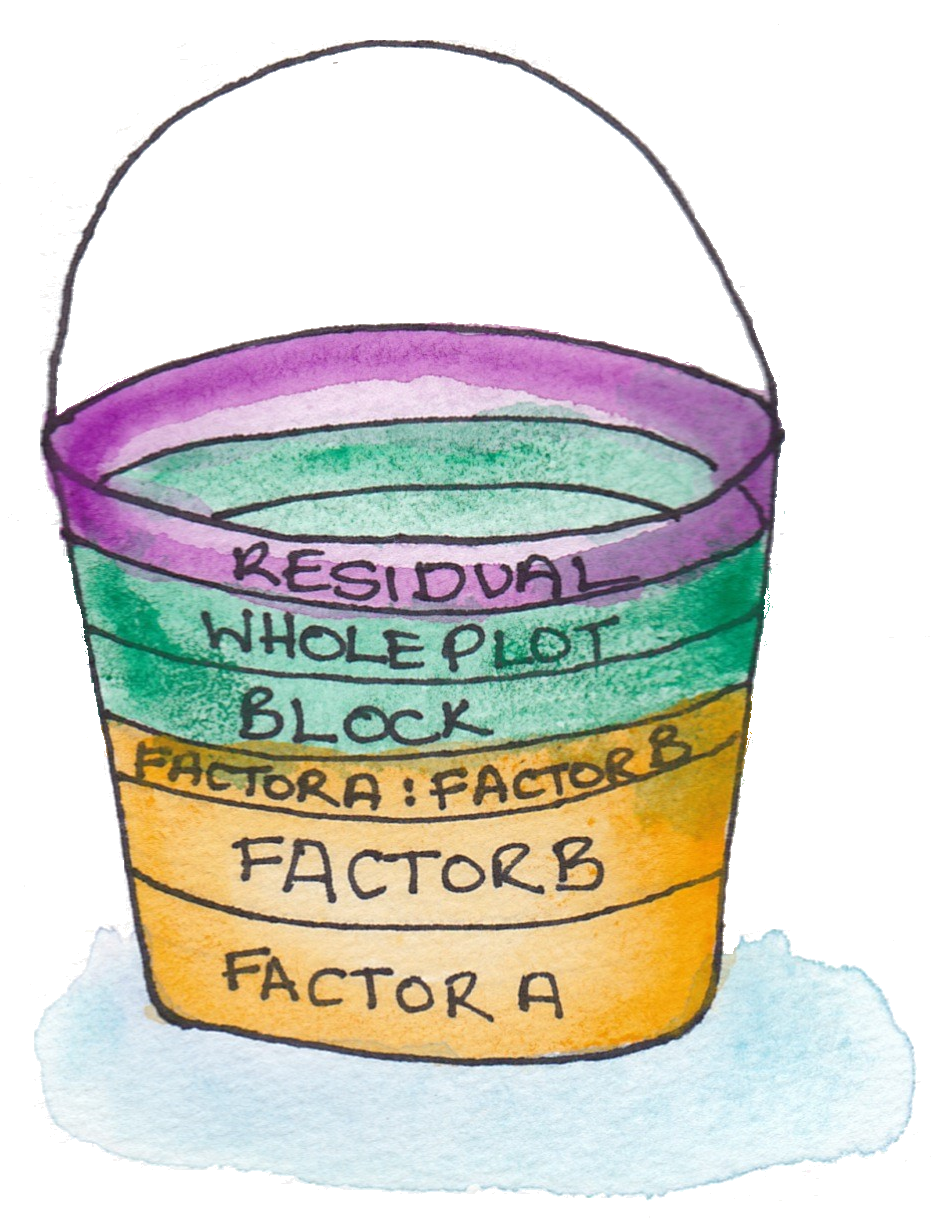
\includegraphics[width = 4cm]{SPBucket.png}
\end{frame}



%%%%%%%%%%%%%%%%%%%%%%%%%%%%%%%%%%%%%%%%%%%%%%%%%%%%%%%%%%%%%%%%%%%%%%%%%%%%%%%%%%%%%%%%%%%%%%%%%%%
% Slide
%%%%%%%%%%%%%%%%%%%%%%%%%%%%%%%%%%%%%%%%%%%%%%%%%%%%%%%%%%%%%%%%%%%%%%%%%%%%%%%%%%%%%%%%%%%%%%%%%%%
\begin{frame}\frametitle{Example 5}
\textit{Grown in 1995-1996 at the Scottish Crop Research Institute.   Split-plot design with 4 blocks,  2 whole-plot
fungicide treatments, and 70 barley varieties or variety mixes.  Total area was 10 rows (north/south) by 56 columns
(east/west).}


It is presumed that the aim of this analysis is to determine if the treatments effect the yield, either as a
combination (interaction) or as a main effect.

\end{frame}


%%%%%%%%%%%%%%%%%%%%%%%%%%%%%%%%%%%%%%%%%%%%%%%%%%%%%%%%%%%%%%%%%%%%%%%%%%%%%%%%%%%%%%%%%%%%%%%%%%%
% Slide
%%%%%%%%%%%%%%%%%%%%%%%%%%%%%%%%%%%%%%%%%%%%%%%%%%%%%%%%%%%%%%%%%%%%%%%%%%%%%%%%%%%%%%%%%%%%%%%%%%%
\begin{frame}\frametitle{Experimental Layout}

\begin{center}
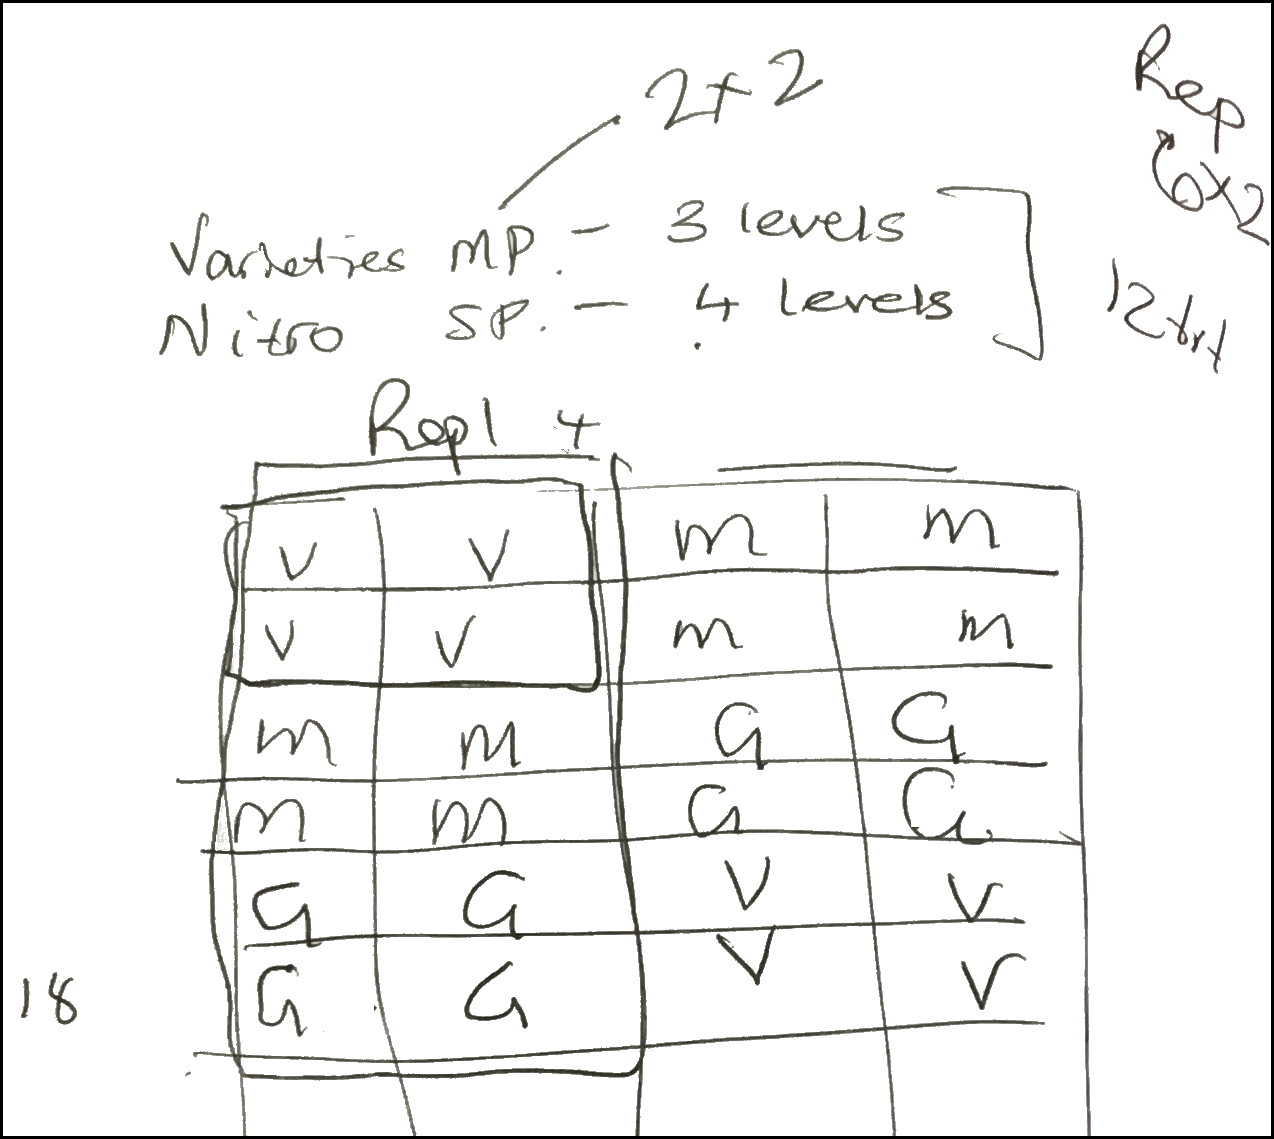
\includegraphics[height = 0.7\textheight]{exptlayout.png}
\end{center}
\flushright

\includegraphics[height = 0.3cm]{yourturn}
\end{frame}


%%%%%%%%%%%%%%%%%%%%%%%%%%%%%%%%%%%%%%%%%%%%%%%%%%%%%%%%%%%%%%%%%%%%%%%%%%%%%%%%%%%%%%%%%%%%%%%%%%%
% Slide
%%%%%%%%%%%%%%%%%%%%%%%%%%%%%%%%%%%%%%%%%%%%%%%%%%%%%%%%%%%%%%%%%%%%%%%%%%%%%%%%%%%%%%%%%%%%%%%%%%%
\begin{frame}\frametitle{Split-plot}
The linear mixed model that is fit can be symbolically written as:
\begin{eqnarray*}
	\texttt{Response variable}&:& \texttt{Yield} \\
	\texttt{Structural component}&:& \texttt{Block, Whole-plot within Block}\\
	\texttt{Explanatory component}&:& \texttt{Genotype, Fungicide}\\
	\texttt{Residual}&:& \texttt{Assume independence}
\end{eqnarray*}

\vspace{1cm}
\flushright

\includegraphics[height = 0.3cm]{yourturn}
\end{frame}

%%%%%%%%%%%%%%%%%%%%%%%%%%%%%%%%%%%%%%%%%%%%%%%%%%%%%%%%%%%%%%%%%%%%%%%%%%%%%%%%%%%%%%%%%%%%%%%%%%%
% Slide
%%%%%%%%%%%%%%%%%%%%%%%%%%%%%%%%%%%%%%%%%%%%%%%%%%%%%%%%%%%%%%%%%%%%%%%%%%%%%%%%%%%%%%%%%%%%%%%%%%%
\begin{frame}\frametitle{Interpreting the output}
Inspection of the residual plots indicates that the model
assumptions are met. Even though there are slight deviations
from a true normal distribution and the Shapiro Wilks
normality test indicates that the residuals are not normally
distributed (p-value < 0.001), the conclusion would be that
the residuals approximately follow a normal distribution.
LMM techniques are robust against departures from normality,
so this would not be considered a serious problem in this
case.

The interaction of Genotype and Fungicide is not significant,
p-value $\ge 0.05$.
\end{frame}

%%%%%%%%%%%%%%%%%%%%%%%%%%%%%%%%%%%%%%%%%%%%%%%%%%%%%%%%%%%%%%%%%%%%%%%%%%%%%%%%%%%%%%%%%%%%%%%%%%%
% Slide
%%%%%%%%%%%%%%%%%%%%%%%%%%%%%%%%%%%%%%%%%%%%%%%%%%%%%%%%%%%%%%%%%%%%%%%%%%%%%%%%%%%%%%%%%%%%%%%%%%%
\begin{frame}\frametitle{Note: none significant interactions}
In this case Genotype and Fungicide are acting independently on Yield, if this were not the case the interaction
term would be significant in the model. When this happens the interaction term is removed from the model and
the model is fit again. Of course the model assumptions will need to be checked again as a different model is
now fitted. The main effects of the model are then assessed for significance.
\end{frame}


%%%%%%%%%%%%%%%%%%%%%%%%%%%%%%%%%%%%%%%%%%%%%%%%%%%%%%%%%%%%%%%%%%%%%%%%%%%%%%%%%%%%%%%%%%%%%%%%%%%
% Slide
%%%%%%%%%%%%%%%%%%%%%%%%%%%%%%%%%%%%%%%%%%%%%%%%%%%%%%%%%%%%%%%%%%%%%%%%%%%%%%%%%%%%%%%%%%%%%%%%%%%
\begin{frame}[fragile]\frametitle{Exercise 13}
\begin{verbatim}
Response: Yield
            Df denDF   F.inc    Pr
(Intercept)  1     5 245.100 0.000
Genotype     2    61   3.809 0.028
Nitrogen     3    61  28.460 0.000

  predicted.value   Genotype std.error groups       ci      low       up
1         97.6250    Victory  7.152596      a 14.28062 83.34438 111.9056
2        104.5000 GoldenRain  7.152596     ab 14.28062 90.21938 118.7806
3        109.7917 Marvellous  7.152596      b 14.28062 95.51105 124.0723

  predicted.value Nitrogen std.error groups      ci       low        up
1        79.38889        0  7.339506      a 14.6538  64.73509  94.04269
2        98.88889      0.2  7.339506      b 14.6538  84.23509 113.54269
3       114.22222      0.4  7.339506      c 14.6538  99.56842 128.87602
4       123.38889      0.6  7.339506      c 14.6538 108.73509 138.04268

\end{verbatim}
\end{frame}

%%%%%%%%%%%%%%%%%%%%%%%%%%%%%%%%%%%%%%%%%%%%%%%%%%%%%%%%%%%%%%%%%%%%%%%%%%%%%%%%%%%%%%%%%%%%%%%%%%%
% Slide
%%%%%%%%%%%%%%%%%%%%%%%%%%%%%%%%%%%%%%%%%%%%%%%%%%%%%%%%%%%%%%%%%%%%%%%%%%%%%%%%%%%%%%%%%%%%%%%%%%%
\begin{frame}[fragile]\frametitle{Exercise 14}
\begin{verbatim}
                   Df denDF  F.inc    Pr
(Intercept)         1     2 48.000 0.020
Variety             4    16  6.943 0.002
Irrigation          1     2 22.820 0.041
Variety:Irrigation  4    16  3.994 0.020

predicted.value Variety Irrigation std.error groups    ci      low       up
1     4.613333 Thumper    Rainfed 0.9902407      a 2.065606 2.547727 6.678939
2     5.470000 Cobbler    Rainfed 0.9902407     ab 2.065606 3.404394 7.535606
3     5.906667   Bravo    Rainfed 0.9902407      b 2.065606 3.841061 7.972273
4     6.193333   Hyola    Rainfed 0.9902407     bc 2.065606 4.127727 8.258939
5     6.433333 Victory    Rainfed 0.9902407     bc 2.065606 4.367727 8.498939
6     6.923333 Thumper  Irrigated 0.9902407     bc 2.065606 4.857727 8.988939
7     7.023333 Victory  Irrigated 0.9902407     bc 2.065606 4.957727 9.088939
8     7.683333   Bravo  Irrigated 0.9902407      c 2.065606 5.617727 9.748939
9     7.703333   Hyola  Irrigated 0.9902407      c 2.065606 5.637727 9.768939
10    7.753333 Cobbler  Irrigated 0.9902407      c 2.065606 5.687727 9.818939

\end{verbatim}
\end{frame}

\section{Extending the model to include spatial modelling}
%%%%%%%%%%%%%%%%%%%%%%%%%%%%%%%%%%%%%%%%%%%%%%%%%%%%%%%%%%%%%%%%%%%%%%%%%%%%%%%%%%%%%%%%%%%%%%%%%%%
% Slide
%%%%%%%%%%%%%%%%%%%%%%%%%%%%%%%%%%%%%%%%%%%%%%%%%%%%%%%%%%%%%%%%%%%%%%%%%%%%%%%%%%%%%%%%%%%%%%%%%%%
\begin{frame}\frametitle{Spatial Analysis}
Up until now we have seen simple linear mixed models in which the random model terms and the residual error term are
all assumed to be independently and identically distributed. We call these variance component models. These models
accommodate broad scale variation in the field but they do not capture small scale variation. Field trial data
typically exhibit local variation (also called plot-to-plot variation or spatial trend). This can be due to moisture
gradients and fertility trends in the field. This results in a higher correlation between plots that are closer to each
spatially.
\end{frame}



%%%%%%%%%%%%%%%%%%%%%%%%%%%%%%%%%%%%%%%%%%%%%%%%%%%%%%%%%%%%%%%%%%%%%%%%%%%%%%%%%%%%%%%%%%%%%%%%%%%
% Slide
%%%%%%%%%%%%%%%%%%%%%%%%%%%%%%%%%%%%%%%%%%%%%%%%%%%%%%%%%%%%%%%%%%%%%%%%%%%%%%%%%%%%%%%%%%%%%%%%%%%
\begin{frame}\frametitle{Spatial Analysis}
In spatial analysis, broad scale variation is accommodated by including appropriate blocking factors as
random terms in the analysis (for example, block in the RCB and both block and row in the LS designs). Alternatively,
spatial variation is accommodated by specifying a more sophisticated spatial covariance structure for the residual
error term. Spatial analysis results in estimated treatment effects that are more accurate and precise than their
counterparts for more traditional methods of analysis.
\end{frame}



%%%%%%%%%%%%%%%%%%%%%%%%%%%%%%%%%%%%%%%%%%%%%%%%%%%%%%%%%%%%%%%%%%%%%%%%%%%%%%%%%%%%%%%%%%%%%%%%%%%
% Slide
%%%%%%%%%%%%%%%%%%%%%%%%%%%%%%%%%%%%%%%%%%%%%%%%%%%%%%%%%%%%%%%%%%%%%%%%%%%%%%%%%%%%%%%%%%%%%%%%%%%
\begin{frame}\frametitle{Spatial Analysis}
Local trend reflects that data for plots that are closer together in the experimental layout are more alike than those
that are further apart. As such, the residuals are correlated, with the correlation being a function of the spatial
distance between the plots.

\textbf{Assumption 1}

It is assumed that the correlation for pairs of plots that are the same distance from each other as the crow flies and
irrespective of where they are positioned in the experimental layout, is the same.

\end{frame}


%%%%%%%%%%%%%%%%%%%%%%%%%%%%%%%%%%%%%%%%%%%%%%%%%%%%%%%%%%%%%%%%%%%%%%%%%%%%%%%%%%%%%%%%%%%%%%%%%%%
% Slide
%%%%%%%%%%%%%%%%%%%%%%%%%%%%%%%%%%%%%%%%%%%%%%%%%%%%%%%%%%%%%%%%%%%%%%%%%%%%%%%%%%%%%%%%%%%%%%%%%%%
\begin{frame}\frametitle{Spatial Analysis}

\textbf{Assumption 2}

Effects can be indexed by columns and rows. The distance between 2 effects is defined by their separation in the column
and row direction, for example, $\varepsilon_{12}$ and $\varepsilon_{35}$ are 2 apart in the row direction and 3 apart
in the column direction. It is assumed that the correlation between 2 smooth trend effects is the product of the
correlation between the column effects of their separation in columns and the correlation between the row effects of
their separation in rows. We call this the assumption of separability. The assumption of separability is
computationally convenient and appears to be reasonable for the two-dimensional smooth trend process associated with
field trials.

\end{frame}



%%%%%%%%%%%%%%%%%%%%%%%%%%%%%%%%%%%%%%%%%%%%%%%%%%%%%%%%%%%%%%%%%%%%%%%%%%%%%%%%%%%%%%%%%%%%%%%%%%%
% Slide
%%%%%%%%%%%%%%%%%%%%%%%%%%%%%%%%%%%%%%%%%%%%%%%%%%%%%%%%%%%%%%%%%%%%%%%%%%%%%%%%%%%%%%%%%%%%%%%%%%%
\begin{frame}\frametitle{Spatial Analysis}
Many forms for modelling the spatial correlation are possible. After the analysis of many hundred field trails, a
separable autoregressive spatial model of order 1 (AR1 $\times$ AR1) is a plausible model for smooth trend in field
trial analysis.

\end{frame}


%%%%%%%%%%%%%%%%%%%%%%%%%%%%%%%%%%%%%%%%%%%%%%%%%%%%%%%%%%%%%%%%%%%%%%%%%%%%%%%%%%%%%%%%%%%%%%%%%%%
% Slide
%%%%%%%%%%%%%%%%%%%%%%%%%%%%%%%%%%%%%%%%%%%%%%%%%%%%%%%%%%%%%%%%%%%%%%%%%%%%%%%%%%%%%%%%%%%%%%%%%%%
\begin{frame}\frametitle{Spatial Analysis}
\textbf{Rule 1}

The number of effects in the residual term must be equal to the number of data units included in the analysis.


\textbf{Rule 2}

Where a compound model term is specified for the residuals, each combination of levels of the factors comprising this
term must uniquely identify one unit of the data.

\textbf{Rule 3}

The data must be ordered to match the R structure specified.

\textbf{Rule 4}

Never fit an autoregressive correlation structure for less than 5 rows or
columns.

\end{frame}


%%%%%%%%%%%%%%%%%%%%%%%%%%%%%%%%%%%%%%%%%%%%%%%%%%%%%%%%%%%%%%%%%%%%%%%%%%%%%%%%%%%%%%%%%%%%%%%%%%%
% Slide
%%%%%%%%%%%%%%%%%%%%%%%%%%%%%%%%%%%%%%%%%%%%%%%%%%%%%%%%%%%%%%%%%%%%%%%%%%%%%%%%%%%%%%%%%%%%%%%%%%%

\begin{frame}\frametitle{Example 6}
A field trial to test the response of a crop to herbicide treatments was
designed as a RCBD with three blocks of 21 plots. The yield at harvest was
recorded for each plot.  The data can be found in \texttt{example6.csv}. Is
there evidence of differences in yield among the herbicide treatments?

\begin{center}
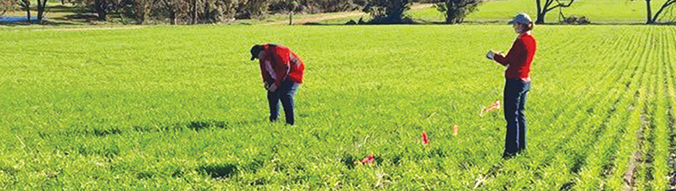
\includegraphics[height = 0.3\textheight]{fieldherb.png}
\end{center}
\end{frame}

%%%%%%%%%%%%%%%%%%%%%%%%%%%%%%%%%%%%%%%%%%%%%%%%%%%%%%%%%%%%%%%%%%%%%%%%%%%%%%%%%%%%%%%%%%%%%%%%%%%
% Slide
%%%%%%%%%%%%%%%%%%%%%%%%%%%%%%%%%%%%%%%%%%%%%%%%%%%%%%%%%%%%%%%%%%%%%%%%%%%%%%%%%%%%%%%%%%%%%%%%%%%
\begin{frame}\frametitle{Experimental Layout}

\begin{center}
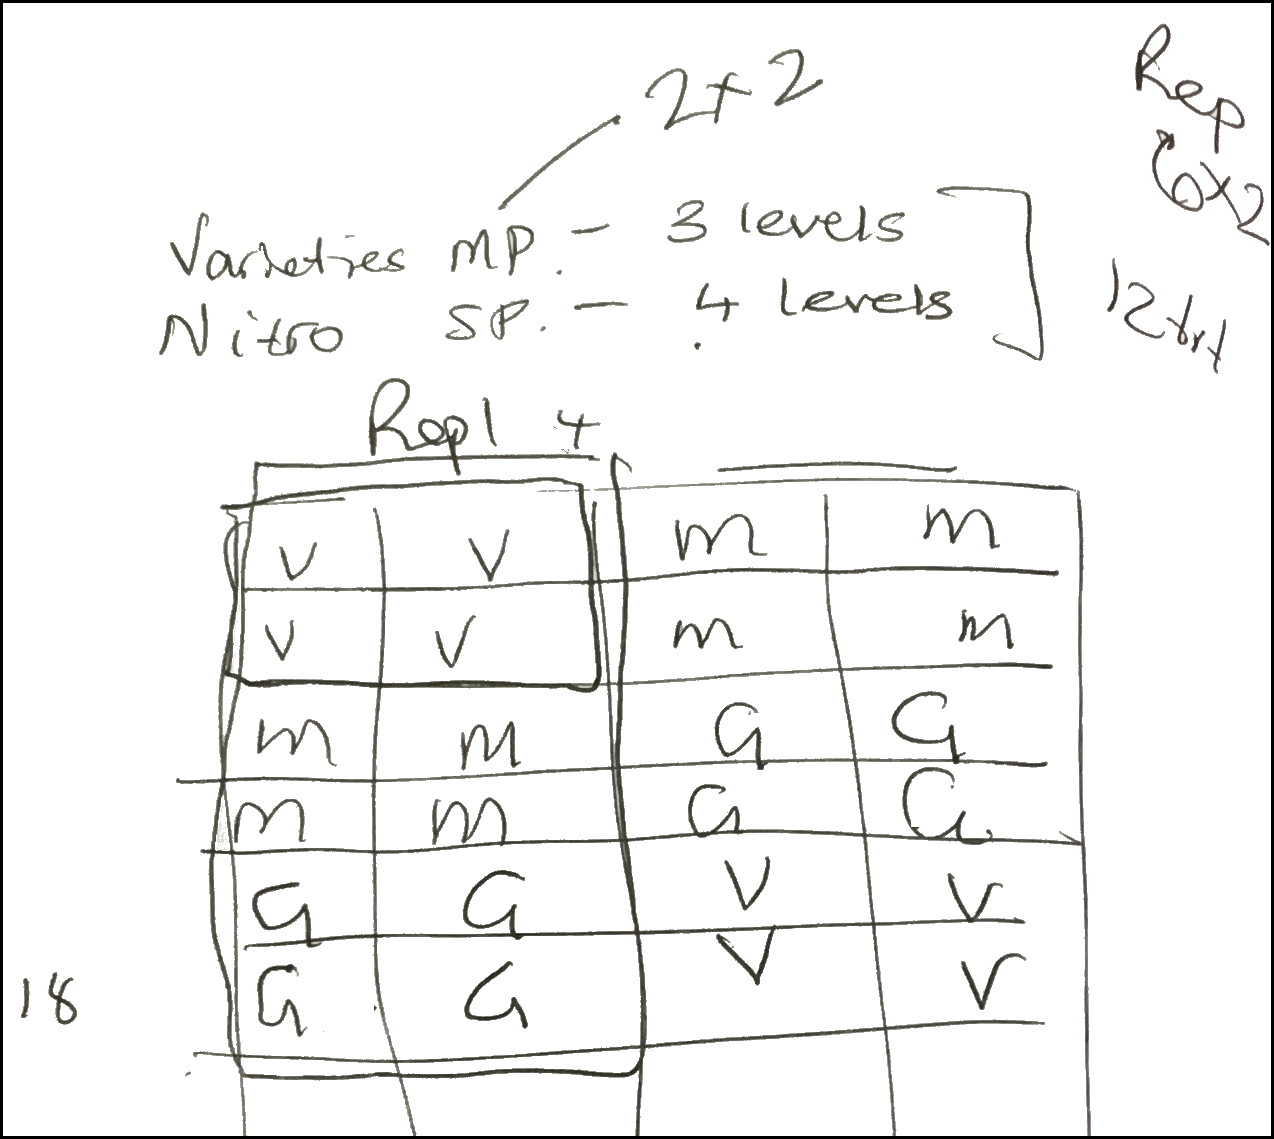
\includegraphics[height = 0.7\textheight]{exptlayout.png}
\end{center}
\flushright

\includegraphics[height = 0.3cm]{yourturn}
\end{frame}

%%%%%%%%%%%%%%%%%%%%%%%%%%%%%%%%%%%%%%%%%%%%%%%%%%%%%%%%%%%%%%%%%%%%%%%%%%%%%%%%%%%%%%%%%%%%%%%%%%%
% Slide
%%%%%%%%%%%%%%%%%%%%%%%%%%%%%%%%%%%%%%%%%%%%%%%%%%%%%%%%%%%%%%%%%%%%%%%%%%%%%%%%%%%%%%%%%%%%%%%%%%%

\begin{frame}\frametitle{Example 6}
The linear model that is fit can be symbolically written as:
\begin{eqnarray*}
	\texttt{Response variable}&:& \texttt{Yield} \\
	\texttt{Structural component}&:& \texttt{Block}\\
	\texttt{Explanatory component}&:& \texttt{Treatment}\\
	\texttt{Residual}&:& \texttt{Explore spatial correlation}
\end{eqnarray*}
\end{frame}


%%%%%%%%%%%%%%%%%%%%%%%%%%%%%%%%%%%%%%%%%%%%%%%%%%%%%%%%%%%%%%%%%%%%%%%%%%%%%%%%%%%%%%%%%%%%%%%%%%%
% Slide
%%%%%%%%%%%%%%%%%%%%%%%%%%%%%%%%%%%%%%%%%%%%%%%%%%%%%%%%%%%%%%%%%%%%%%%%%%%%%%%%%%%%%%%%%%%%%%%%%%%

\begin{frame}[fragile]\frametitle{Exercise 15}
\begin{verbatim}
                  Df denDF   F.inc    Pr
(Intercept)        1   5.5 247.200 0.000
Genotype           2  55.4   4.069 0.022
Nitrogen           3  42.9  45.030 0.000
Genotype:Nitrogen  6  41.4   0.465 0.830

  predicted.value   Genotype std.error groups       ci      low       up
1        97.80461    Victory  7.206781      a 14.38880 83.41580 112.1934
2       102.57666 GoldenRain  7.264648     ab 14.50434 88.07232 117.0810
3       109.27679 Marvellous  7.175646      b 14.32664 94.95015 123.6034

  predicted.value Nitrogen std.error groups       ci       low        up
1        77.08206        0  7.251809      a 14.47870  62.60335  91.56076
2        98.47013      0.2  7.209918      b 14.39506  84.07507 112.86519
3       114.44260      0.4  7.198464      c 14.37220 100.07040 128.81479
4       122.88263      0.6  7.224191      c 14.42356 108.45906 137.30619

\end{verbatim}

\end{frame}


%%%%%%%%%%%%%%%%%%%%%%%%%%%%%%%%%%%%%%%%%%%%%%%%%%%%%%%%%%%%%%%%%%%%%%%%%%%%%%%%%%%%%%%%%%%%%%%%%%%
% Slide
%%%%%%%%%%%%%%%%%%%%%%%%%%%%%%%%%%%%%%%%%%%%%%%%%%%%%%%%%%%%%%%%%%%%%%%%%%%%%%%%%%%%%%%%%%%%%%%%%%%

\begin{frame}[fragile]\frametitle{Exercise 16}
\begin{verbatim}
            Df denDF   F.inc Pr
(Intercept)  1  12.2 273.300  0
Genotype    49  80.9   4.783  0

   predicted.value Genotype std.error   groups        ci      low       up
1         1.531944      G36 0.2764750       ab 0.5485185 0.983426 2.080463
2         1.590845      G28 0.2747931       ac 0.5451817 1.045663 2.136027
3         1.808187      G07 0.2701121     abce 0.5358947 1.272293 2.344082
4         1.874460      G46 0.2687801    abcef 0.5332521 1.341208 2.407712
5         1.884487      G29 0.2684802    abcef 0.5326571 1.351829 2.417144
6         1.886878      G43 0.2685921    abcef 0.5328791 1.353999 2.419757
\end{verbatim}

\end{frame}


\section{Modelling complex treatment structures}
%%%%%%%%%%%%%%%%%%%%%%%%%%%%%%%%%%%%%%%%%%%%%%%%%%%%%%%%%%%%%%%%%%%%%%%%%%%%%%%%%%%%%%%%%%%%%%%%%%%
% Slide
%%%%%%%%%%%%%%%%%%%%%%%%%%%%%%%%%%%%%%%%%%%%%%%%%%%%%%%%%%%%%%%%%%%%%%%%%%%%%%%%%%%%%%%%%%%%%%%%%%%
\begin{frame}\frametitle{Modelling complex treatment structures}

In the design workshop we saw that it was possible to plan experiments with more than one treatment variable. We have
seen the analysis of a split-plot experiment where there was a factorial treatment structure with two explanatory
variables. There are other more complex treatment structures that can be used when analysing experimental data.

\end{frame}


%%%%%%%%%%%%%%%%%%%%%%%%%%%%%%%%%%%%%%%%%%%%%%%%%%%%%%%%%%%%%%%%%%%%%%%%%%%%%%%%%%%%%%%%%%%%%%%%%%%
% Slide
%%%%%%%%%%%%%%%%%%%%%%%%%%%%%%%%%%%%%%%%%%%%%%%%%%%%%%%%%%%%%%%%%%%%%%%%%%%%%%%%%%%%%%%%%%%%%%%%%%%
\begin{frame}\frametitle{Modelling complex treatment structures}
For example, Example 6 had 21 herbicide treatments, one of which was a control. The treatments were:
\begin{multicols}{2}
\begin{enumerate}
\item  Achieve\_250g
\item  Achieve\_300g
\item  Achieve\_380g
\item  Atlantis\_300mL
\item  Atlantis\_330mL
\item  Control\_0
\item  Hoegrass\_0.75L
\item  Hoegrass\_1.0L
\item  Hoegrass\_1.2L
\item  Hussar\_150g
\item  Hussar\_200g
\item  MatavenL\_2.25L
\item  MatavenL\_3.0L
\item  Topik\_50mL
\item  Topik\_65mL
\item  Topik\_85mL
\item  Tristar\_1.0L
\item  Tristar\_1.5L
\item  Wildcat\_250mL
\item  Wildcat\_300mL
\item  Wildcat\_350mL
\end{enumerate}
\end{multicols}
\end{frame}


%%%%%%%%%%%%%%%%%%%%%%%%%%%%%%%%%%%%%%%%%%%%%%%%%%%%%%%%%%%%%%%%%%%%%%%%%%%%%%%%%%%%%%%%%%%%%%%%%%%
% Slide
%%%%%%%%%%%%%%%%%%%%%%%%%%%%%%%%%%%%%%%%%%%%%%%%%%%%%%%%%%%%%%%%%%%%%%%%%%%%%%%%%%%%%%%%%%%%%%%%%%%
\begin{frame}\frametitle{Example 6}
The simple hypothesis was tested:

\begin{eqnarray*}
	H_0&:& \texttt{Yield is the same for all Treatments} \\
	H_1&:& \texttt{Yield is not the same for all Treatments}
\end{eqnarray*}

It can be seen that the 21 treatments are made up of 8 different herbicides with 2 or 3 different rates of application
within a herbicide. This treatment structure would have been purposefully made.
\end{frame}


%%%%%%%%%%%%%%%%%%%%%%%%%%%%%%%%%%%%%%%%%%%%%%%%%%%%%%%%%%%%%%%%%%%%%%%%%%%%%%%%%%%%%%%%%%%%%%%%%%%
% Slide
%%%%%%%%%%%%%%%%%%%%%%%%%%%%%%%%%%%%%%%%%%%%%%%%%%%%%%%%%%%%%%%%%%%%%%%%%%%%%%%%%%%%%%%%%%%%%%%%%%%
\begin{frame}\frametitle{Example 6}

\begin{eqnarray*}
	H_0&:& \texttt{Yield is the same for the Control and the Treatments} \\
	H_1&:& \texttt{Yield is not the same for the Control and the Treatments}
\end{eqnarray*}

\begin{eqnarray*}
	H_0&:& \texttt{Yield is not affected by the different Herbicide Treatments} \\
	H_1&:& \texttt{Yield is affected by the different Herbicide Treatments}
\end{eqnarray*}

\begin{eqnarray*}
	H_0&:& \texttt{Yield is not affected differently by rate of application within} \\
&& \texttt{the Herbicide Treatments} \\
	H_1&:& \texttt{Yield is affected differently by rate of application within the} \\
&&\texttt{Herbicide Treatments}
\end{eqnarray*}

\end{frame}


%%%%%%%%%%%%%%%%%%%%%%%%%%%%%%%%%%%%%%%%%%%%%%%%%%%%%%%%%%%%%%%%%%%%%%%%%%%%%%%%%%%%%%%%%%%%%%%%%%%
% Slide
%%%%%%%%%%%%%%%%%%%%%%%%%%%%%%%%%%%%%%%%%%%%%%%%%%%%%%%%%%%%%%%%%%%%%%%%%%%%%%%%%%%%%%%%%%%%%%%%%%%
\begin{frame}\frametitle{Example 6}
To fit a model to answer these three hypotheses the data must contain a separate columns for Control (Yes/No),
Herbicide (Achieve, Atlantis, Control, Hoegrass, Hussar, MatavenL, Topik, Tristar \& Wildcat) and Application Rate.
Each column relates to each of the hypotheses.

\begin{center}
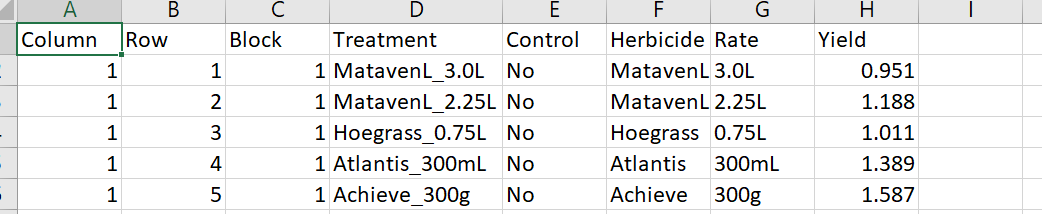
\includegraphics[height = 0.3\textheight]{complextrt.png}
\end{center}

\end{frame}


%%%%%%%%%%%%%%%%%%%%%%%%%%%%%%%%%%%%%%%%%%%%%%%%%%%%%%%%%%%%%%%%%%%%%%%%%%%%%%%%%%%%%%%%%%%%%%%%%%%
% Slide
%%%%%%%%%%%%%%%%%%%%%%%%%%%%%%%%%%%%%%%%%%%%%%%%%%%%%%%%%%%%%%%%%%%%%%%%%%%%%%%%%%%%%%%%%%%%%%%%%%%
\begin{frame}\frametitle{Example 6}
The linear model that is fit can be symbolically written as:
\begin{eqnarray*}
	\texttt{Response variable}&:& \texttt{Yield} \\
	\texttt{Structural component}&:& \texttt{Block}\\
	\texttt{Explanatory component}&:& \texttt{Control, Herbicide, Herbicide:Rate}
\end{eqnarray*}
The modelling process is altered by fitting an AR1 $\times$ ID process to accommodate a smooth spatial trend.

\end{frame}

%%%%%%%%%%%%%%%%%%%%%%%%%%%%%%%%%%%%%%%%%%%%%%%%%%%%%%%%%%%%%%%%%%%%%%%%%%%%%%%%%%%%%%%%%%%%%%%%%%%
% Slide
%%%%%%%%%%%%%%%%%%%%%%%%%%%%%%%%%%%%%%%%%%%%%%%%%%%%%%%%%%%%%%%%%%%%%%%%%%%%%%%%%%%%%%%%%%%%%%%%%%%
\begin{frame}[fragile]\frametitle{Exercise 17}
\begin{verbatim}
            Df denDF  F.inc    Pr
(Intercept)  1   4.7 64.960 0.001
Control      1  16.9 22.230 0.000
Season       1  17.9  6.816 0.018
Rate         2  16.8  4.595 0.026

  predicted.value Control std.error groups       ci      low       up
1        12.05221      No  1.871703      a 3.840417  8.21179 15.89262
2        22.84462     Yes  2.452749      b 5.032625 17.81199 27.87724

1        9.158917      F  2.132531      a 4.375593  4.783324 13.53451
2       14.945498      S  2.200014      b 4.514057 10.431441 19.45955
3       22.844618      O  2.452749      c 5.032625 17.811994 27.87724

1        7.813065   12  2.398790      a 4.921911  2.891154 12.73498
2       14.087980    6  2.410639      a 4.946222  9.141758 19.03420
3       14.255578    3  2.370603      a 4.864076  9.391502 19.11965
4       22.844618    0  2.452749      b 5.032625 17.811994 27.87724
\end{verbatim}
\end{frame}


%%%%%%%%%%%%%%%%%%%%%%%%%%%%%%%%%%%%%%%%%%%%%%%%%%%%%%%%%%%%%%%%%%%%%%%%%%%%%%%%%%%%%%%%%%%%%%%%%%%
% Slide
%%%%%%%%%%%%%%%%%%%%%%%%%%%%%%%%%%%%%%%%%%%%%%%%%%%%%%%%%%%%%%%%%%%%%%%%%%%%%%%%%%%%%%%%%%%%%%%%%%%
\begin{frame}\frametitle{References}
\bibliographystyle{apacite}
\bibliography{ref2}
\end{frame}


\end{document}
